% arara: pdflatex
% arara: pdflatex
% arara: biber
% arara: pdflatex
% arara: pdflatex
% arara: clean: { files: [ arara-usermanual.aux, arara-usermanual.bbl ] }
% arara: clean: { files: [ arara-usermanual.bcf, arara-usermanual.cod ] } 
% arara: clean: { files: [ arara-usermanual.blg, arara-usermanual.lof ] }
% arara: clean: { files: [ arara-usermanual.lot, arara-usermanual.out ] } 
% arara: clean: { files: [ arara-usermanual.toc, arara-usermanual.log ] } 
% arara: clean: { files: [ arara-usermanual.run.xml ] }
% -------------------------------------------------
% Arara -- the cool TeX automation tool
% Copyright (c) 2012, Paulo Roberto Massa Cereda
% All rights reserved.
%
% Redistribution and  use in source  and binary forms, with  or without
% modification, are  permitted provided  that the  following conditions
% are met:
%
% 1. Redistributions  of source  code must  retain the  above copyright
% notice, this list of conditions and the following disclaimer.
%
% 2. Redistributions in binary form  must reproduce the above copyright
% notice, this list  of conditions and the following  disclaimer in the
% documentation and/or other materials provided with the distribution.
%
% 3. Neither  the name  of the  project's author nor  the names  of its
% contributors may be used to  endorse or promote products derived from
% this software without specific prior written permission.
%
% THIS SOFTWARE IS  PROVIDED BY THE COPYRIGHT  HOLDERS AND CONTRIBUTORS
% "AS IS"  AND ANY  EXPRESS OR IMPLIED  WARRANTIES, INCLUDING,  BUT NOT
% LIMITED  TO, THE  IMPLIED WARRANTIES  OF MERCHANTABILITY  AND FITNESS
% FOR  A PARTICULAR  PURPOSE  ARE  DISCLAIMED. IN  NO  EVENT SHALL  THE
% COPYRIGHT HOLDER OR CONTRIBUTORS BE  LIABLE FOR ANY DIRECT, INDIRECT,
% INCIDENTAL, SPECIAL, EXEMPLARY,  OR CONSEQUENTIAL DAMAGES (INCLUDING,
% BUT  NOT LIMITED  TO, PROCUREMENT  OF SUBSTITUTE  GOODS OR  SERVICES;
% LOSS  OF USE,  DATA, OR  PROFITS; OR  BUSINESS INTERRUPTION)  HOWEVER
% CAUSED AND  ON ANY THEORY  OF LIABILITY, WHETHER IN  CONTRACT, STRICT
% LIABILITY, OR TORT (INCLUDING NEGLIGENCE OR OTHERWISE) ARISING IN ANY
% WAY  OUT  OF  THE USE  OF  THIS  SOFTWARE,  EVEN  IF ADVISED  OF  THE
% POSSIBILITY OF SUCH DAMAGE.
% -------------------------------------------------

\documentclass[a4paper,twoside,12pt]{memoir}

% packages
% -------------------------------------------------
\usepackage[T1]{fontenc}
\usepackage[utf8]{inputenc}
\usepackage{arara}
% -------------------------------------------------

% bibliography
% -------------------------------------------------
\addbibresource{references.bib}
% -------------------------------------------------

% current version
% -------------------------------------------------
\newcommand{\araraversion}{3.0}
% -------------------------------------------------

% document
% -------------------------------------------------
\begin{document}

% title page
% -------------------------------------------------
\begin{titlingpage}

\begin{center}
\vspace*{2em}

\scalebox{1.15}{\araralogo}

\vspace{2em}

{\color{araracolor}\fontfamily{fco}\bfseries\Huge The cool \TeX{} automation tool}

\vspace{10em}

{\Huge\sffamily\bfseries User Manual}

\vspace{3em}

{\large
\tabcolsep=1em
\begin{tabular}{cc}
\multicolumn{2}{c}{Paulo R.\ M.\ Cereda}\\
\multicolumn{2}{c}{\url{cereda@users.sf.net}}\\[1.5em]
Marco Daniel & Brent Longborough\\
\url{marco.daniel@mada-nada.de} & \url{brent@longborough.org}
\end{tabular}}

\vfill

{\LARGE\sffamily\bfseries Version \araraversion}

\end{center}

\end{titlingpage}
% -------------------------------------------------

% set styles
% -------------------------------------------------
\chapterstyle{madsen}
\pagestyle{headings} 
\frontmatter
\nouppercaseheads
% -------------------------------------------------

% Prologue
% -------------------------------------------------
\chapter*{Prologue}
\label{chap:prologue}

\epigraph{\emph{Moral of the story: never read the documentation, bad things happen.}}{David Carlisle}

When I released the very first version of \arara on a Friday 13th, April 2012, I never thought the tool would
receive so many positive comments and feedback. To be honest, since \arara was written for helping me
with my own personal \LaTeX\ projects, I really doubted if the tool could be of service to anyone else. And,
to my surprise, it seems \arara did good. To a lot of people around the \TeX\ world.

I never intended to release the tool to the whole world, since I wasn't sure if other people could benefit from
\arara's features. After all, there's already a plethora of tools available to the \TeX\ community in general,
although with different approaches. The reason I decided to make \arara publicly available is quite simple:
I wanted to somehow contribute to the \TeX\ community, and I wanted to give my best to make such
community even more awesome.

As time goes by, I'm quite satisfied with the current state of \arara~--~this is our 3rd major release. We
have reached a very mature code and a great team of developers, translators and testers. Since version 1.0,
the code evolved a lot -- new features, lots of bug fixes, improvements -- thanks to all the feedback I
received. In my humble opinion, that's how any project should evolve: based on what our users expect and
want to achieve. I'm proud to see \arara being 100\% community-driven, it's a big achievement for a project
with less than one year old.

First of all, I'd like to thank some friends of mine that really made \arara possible: Alan Munn, for providing
great ideas and suggestions to the manual; Andrew Stacey, for heavily testing \arara, providing great user
cases, and for suggesting improvements to the program; Brent Longborough, a member of the core team,
for providing great suggestions and ideas to the program logic, writing rules, testing the code and also for
working with the Portuguese and Turkish translations; Clemens Niederberger, for testing \arara, and also
writing a great tutorial about it in his
\href{http://www.mychemistry.eu/2012/06/arara-automate-latex-birds-music/}{blog on chemistry and \LaTeX};
David Carlisle, for reminding me to work on \arara, and also encouraging me to write answers about it in
our \TeX\ community; Enrico Gregorio, for reviewing the original manual, testing \arara, providing great
ideas and suggestions to the manual and to the program itself, and for working with the Italian translation;
Francesco Endrici, for providing the very first \arara rule outside our core team; Harish Kumar, for being a
heavy \arara user and integrating it with WinEdt and Inlage; \.Ilhan Polat for working with Brent in the Turkish
translation; Joseph Wright, for testing it, providing contributed code for Linux and Mac installations, and also
blogging about \arara in his \href{http://www.texdev.net}{personal blog}; Gonzalo Medina, for providing the
Spanish translation; Mikaël Maunier, for providing the French translation; Marco Daniel, one of core team
members, for heavily testing \arara, suggesting enhancements to the manual and to the program itself,
providing lots of contributed rules for common tasks, and also for the German version; Patrick Gundlach,
for advertising \arara in the official Twitter channel of \href{http://www.dante.de}{Dante} -- the German
\TeX\ User Group; Stefan Kottwitz, for encouraging me to write an article about \arara, published in the
\href{http://latex-community.org/know-how/435-gnuplot-arara}{\LaTeX\ Community} forum, and also
tweeting about it. Thank you very much. I'm sorry if I forgot to mention somebody, I really have so much
people to thank and my memory happens to be very short.

That said, I still believe that the warning featured in the first version of this manual still applies:
\textsc{Hic Sunt Dracones}. Though the code really evolved from the first commit I made, \arara is far from
being bug-free. And you will learn that \arara gives you enough rope. In other words, \emph{you} will be
responsible for how \arara behaves and all the consequences from your actions. Sorry to sound scary, but I
really needed to tell you this. After all, one of \arara's greatest features is the freedom it offers. But as you
know, freedom always comes at a cost. Please, don't send us angry letters -- or e-mails, perhaps -- if
something bad happen.

Feedback is surely welcome for me to improve this humble tool, just write an e-mail to me or any other
member of the team and we will reply as soon as possible. The source code is fully available at
\url{http://github.com/cereda/arara}, feel free to contribute to the project by forking it, submitting bugs,
sending pull requests or even translating it to your language. If you want to support the \LaTeX\ development
by a donation, the best way to do this is donating to the \href{http://www.tug.org/}{\TeX\ Users Group}.
Please also  consider joining our \TeX\ community at \href{http://tex.stackexchange.com}{StackExchange}.

\vspace{2em}

\begin{flushright}
Paulo Roberto Massa Cereda\\
\emph{on behalf of the \arara team}
\end{flushright}

%\vspace{8em}
\vfill

\begin{center}
\scalebox{0.55}{\araralogo}

\vspace{0.3em}

{\color{araracolor}\fontfamily{fco}\bfseries\large Proudly made on Earth}
\end{center}
% -------------------------------------------------

\cleardoublepage

% Special thanks
% -------------------------------------------------
\section*{Special thanks}

\begin{mdframed}[roundcorner=10pt,linecolor=araracolor,middlelinewidth=1pt]
\centering
{\renewcommand{\arraystretch}{1.5}
\sffamily
\begin{tabular}{ccc}
Alan Munn & Andrew Stacey & Brent Longborough\\
Clemens Niederberger & David Carlisle & Enrico Gregorio\\
Francesco Endrici & Harish Kumar & \.Ilhan Polat\\
Joseph Wright & Gonzalo Medina & Mikaël Maunier\\
Marco Daniel & Patrick Gundlach & Stefan Kottwitz
\end{tabular}}
\end{mdframed}

\vspace{1em}

\noindent\arara also makes use of some specific opensource Java projects and libraries in order to properly
work. I would like to thank the following projects and their respective developers:

\begin{enumerate}
\item \href{http://commons.apache.org}{Apache Commons}, a project from the Apache Foundation focused
on all aspects of reusable Java components. \arara uses three of the Commons libraries:
\href{http://commons.apache.org/cli/}{CLI}, which provides a command line arguments parser,
\href{http://commons.apache.org/collections/}{Collections}, a library which extends the Java Collections
Framework, and \href{http://commons.apache.org/exec/}{Exec}, an API for dealing with external process
execution and environment management in Java.

\item \href{http://logback.qos.ch}{Logback}, a logging framework intended to be the successor to the
popular \href{http://logging.apache.org/log4j/}{log4j} project. According to some benchmarks, it is faster
and has a smaller footprint than all existing logging systems, sometimes by a wide margin.

\item \href{http://code.google.com/p/snakeyaml}{SnakeYAML}, a YAML parser and emitter for the Java
programming language. YAML is a data serialization format designed for human readability and interaction
with scripting languages. \arara uses YAML as the rule format.

\item \href{http://www.slf4j.org/}{SLF4J}, a simple facade or abstraction for various logging frameworks,
allowing the end user to plug in the desired logging framework at deployment time.

\item \href{http://mvel.codehaus.org}{MVEL}, a powerful expression language for Java-based applications.
It provides a plethora of features and is suited for everything from the smallest property binding and extraction,
to full blown scripts. \arara relies on MVEL to provide the expansion mechanism for rules.

\item \href{http://maven.apache.org/}{Apache Maven}, a software project management and comprehension tool.
Based on the concept of a project object model, Maven can manage a project's build, reporting and documentation
from a central piece of information. 

\item \href{http://izpack.github.com}{IzPack}, a Java-based software installer builder that will run on any
operating system coming with a Java Virtual Machine that is compliant with the Oracle JVM 1.5 or higher.
\end{enumerate}

A special thanks goes to my great friend \href{http://antoineneveux.fr/}{Antoine Neveux} for encouraging me to
try out the \href{http://maven.apache.org}{Apache Maven} software project management. In the past, \arara was
released as a NetBeans project, which is based on \href{http://ant.apache.org/}{Apache Ant}, another great tool
from the Apache Foundation. Although I'm really fine with Ant, thanks to Maven, now it is way easier to build and
to maintain the code. And it's always nice to learn another tool.

And at last but not least, I want to thank you, dear reader and potential user, for giving \arara a try. Do not despair
if you don't succeed with \arara at first; just try again. I'm sure you will find your way. This humble project is
opensource and it will always be. Let the bird be your guide through the journey to the typographic land. Have a
good read.
% -------------------------------------------------

\cleardoublepage

% Release information
% -------------------------------------------------
\section*{Release information}

\subsection*{Version 3.0}
\begin{itemize}
\item[\newfeature] 
     % TODO
     List of new features and a table containing the lines of code for
     version 3.0.
\end{itemize}

{\renewcommand{\arraystretch}{1.5}
\begin{table}[ht]
\centering
\caption{Lines of code for version 3.0.}
\begin{tabular}{lrrrr}
\hline
\textbf{Language} & \textbf{Files} & \textbf{Blank} & \textbf{Comment} & \textbf{Code}\\
\hline
\hline
Java & 0 & 0 & 0 & 0\\
XML & 0 & 0 & 0 & 0\\
\hline
Sum & 0 & 0 & 0 & 0\\
\hline
\end{tabular}
\label{tab:locarara30}
\end{table}}

\subsection*{Version 2.0}
\begin{itemize}
\item[\newfeature] 
     Added the |--timeout n| flag to allow setting a timeout for every task. If
     the timeout is reached before the task ends, \arara will kill it and 
     interrupt the processing. The $n$ value is expressed in milliseconds.
\item[\bugfix] 
     Fixed the |--verbose| flag to behave as a realtime output.
\item[\newfeature] 
     There's no need of noninteractive commands anymore. \arara can now handle
     user input through the |--verbose| tag. If the flag is not set and the 
     command requires user interaction, the task execution is interrupted.
\item[\bugfix] 
     Fixed the execution of some script-based system commands to ensure 
     cross-platform compatibility.
\item[\newfeature] 
     Added the |@{SystemUtils}| orb tag to provide specific operating system 
     checks. The orb tag maps the |SystemUtils| class from the amazing 
     \href{http://commons.apache.org/lang/}{Apache Commons Lang} library and 
     all of its methods and properties.
\end{itemize}

{\renewcommand{\arraystretch}{1.5}
\begin{table}[ht]
\centering
\caption{Lines of code for version 2.0.}
\begin{tabular}{lrrrr}
\hline
\textbf{Language} & \textbf{Files} & \textbf{Blank} & \textbf{Comment} & \textbf{Code}\\
\hline
\hline
Java & 20 & 608 & 1642 & 848\\
XML & 1 & 0 & 0 & 12\\
\hline
Sum & 21 & 608 & 1642 & 860\\
\hline
\end{tabular}
\label{tab:locarara20}
\end{table}}

\subsection*{Version 1.0.1}

\begin{itemize}
\item[\newfeature] 
     Added support for |.tex|, |.dtx| and |.ltx| files. When no extension is 
     provided, \arara will automatically look for these extensions in this 
     specific order.
\item[\newfeature] 
     Added the |--verbose| flag to allow printing the complete log in the 
     terminal. A short |-v| tag is also available. Both |stdout| and |stderr| 
     are printed.
\item[\bugfix] 
     Fixed exit status when an exception is thrown. Now \arara also returns a 
     non-zero exit status when something wrong happened. Note that this 
     behaviour happens only when \arara is processing a file.
\end{itemize}

{\renewcommand{\arraystretch}{1.5}
\begin{table}[ht]
\centering
\caption{Lines of code for version 1.0.1.}
\begin{tabular}{lrrrr}
\hline
\textbf{Language} & \textbf{Files} & \textbf{Blank} & \textbf{Comment} & \textbf{Code}\\
\hline
\hline
Java & 20 & 585 & 1671 & 804\\
XML & 1 & 0 & 6 & 12\\
\hline
Sum & 21 & 585 & 1677 & 816\\
\hline
\end{tabular}
\label{tab:locarara101}
\end{table}}

\subsection*{Version 1.0}

\begin{itemize}
\item[\newfeature] First public release.
\end{itemize}

{\renewcommand{\arraystretch}{1.5}
\begin{table}[ht]
\centering
\caption{Lines of code for version 1.0.}
\begin{tabular}{lrrrr}
\hline
\textbf{Language} & \textbf{Files} & \textbf{Blank} & \textbf{Comment} & \textbf{Code}\\
\hline
\hline
Java & 20 & 524 & 1787 & 722\\
XML & 1 & 0 & 6 & 12\\
\hline
Sum & 21 & 524 & 1793 & 734\\
\hline
\end{tabular}
\label{tab:locarara10}
\end{table}}
% -------------------------------------------------

\cleardoublepage

% License
% -------------------------------------------------
\section*{License}
\label{sec:license}

\arara is licensed under the 
\href{http://www.opensource.org/licenses/bsd-license.php}{New BSD License}. It's
important to observe that the New BSD License has been verified as a 
GPL-compatible free software license by the 
\href{http://www.fsf.org/}{Free Software Foundation}, and has been vetted as an 
open source license by the 
\href{http://www.opensource.org/}{Open Source Initiative}.

\vspace{1.5em}

\ornamentline

\vfill

\begin{mdframed}[roundcorner=10pt,linecolor=araracolor,middlelinewidth=1pt]
\noindent
\begingroup
  \color{araracolor}\fontfamily{fco}\bfseries
  \arara \ -- the cool \TeX{} automation tool
\endgroup

\vspace{.5em}

\noindent Copyright \copyright{} 2012, Paulo Roberto Massa Cereda

\noindent All rights reserved.

\vspace{1em}

\noindent Redistribution and use in source and binary forms, with or without
modification, are permitted provided that the following conditions are met:

\vspace{1em}

\begin{itemize}
\item Redistributions of source code must retain the above copyright notice, 
      this list of conditions and the following disclaimer.
\item Redistributions in binary form must reproduce the above copyright notice,
      this list of conditions and the following disclaimer in the documentation
      and/or other materials provided with the distribution.
\end{itemize}

\vspace{1em}

\noindent\textsc{This software is provided by the copyright holders and 
contributors ``as is'' and any express or implied warranties, including, but not
 limited to, the implied warranties of merchantability and fitness for a 
particular purpose are disclaimed. In no event shall the copyright holder or 
contributors be liable for any direct, indirect, incidental, special, exemplary,
 or consequential damages (including, but not limited to, procurement of 
substitute goods or services; loss of use, data, or profits; or business 
interruption) however caused and on any theory of liability, whether in contract,
 strict liability, or tort (including negligence or otherwise) arising in any 
way out of the use of this software, even if advised of the possibility of such
damage.}
\end{mdframed}
% -------------------------------------------------

\cleardoublepage

\vspace*{25em}

\begin{flushright}
\em To my cat Fubá, who loves birds.
\end{flushright}

\cleardoublepage

% TOC and list of codes
% -------------------------------------------------
\tableofcontents*

\cleardoublepage

\listoffigures*

\cleardoublepage

\listoftables*

\cleardoublepage

\listofcodes*
% -------------------------------------------------

\mainmatter

\part{The application}
\label{part:application}

\chapter{Introduction}
\label{chap:introduction}

\epigraph{\emph{You can do such a lot with a Wompom, you can use every part of it too.
For work or for pleasure, it's a triumph, it's a treasure,
oh there's nothing that a Wompom cannot do.}}{Flanders \& Swann}

Hello there, welcome to \arara! I'm glad you were not intimidated by the threatening
message in the prologue. This chapter is actually a quick introduction to what you
can expect from \arara. Don't be afraid, it will be easy to digest, I promise.

\section{What is \texorpdfstring{\arara}{arara}?}
\label{sec:whatisarara}

Good question! \arara is a \TeX\ automation tool based on rules and directives. It is,
in some aspects, similar to other well-known tools like |latexmk|~\cite{collins:2001}
and |rubber|~\cite{rubber:2009}. The key difference might be the fact that \arara
aims at explicit instructions in the source code in order to determine what to do instead
of relying on other resources, such as log file analysis. It's a different approach for an automation tool, and
we have both advantages and disadvantages of such decision. Let's talk about
disadvantages first.

Since we need to explicitly tell \arara what we want it to do, it might not be intuitive
for casual users. Tools like |latexmk| and |rubber| rely on a analysis scheme in which
the document is generated with a simple call to |latexmk mydoc.tex| or |rubber --pdf mydoc.tex|,
while a similar call to |arara mydoc.tex| does absolutely nothing; it's not wrong, it's by design:
\arara needs to know what you want. We do this by adding a directive in our |.tex| file, as shown
in line~1 of Code~\ref{code:hellolatex}. Don't worry with the terms now, we will come back to the
concepts later on in this manual, in Chapter~\ref{chap:importantconcepts}.

\begin{code}[htbp]
\caption{\mycmd{mydoc.tex}}
\label{code:hellolatex}
\begin{latex}
% (*@@*)arara: pdflatex
\documentclass{article}

\begin{document}
Hello world.
\end{document}
\end{latex}
\end{code}

When we add a directive in our source code, we are explicitly telling \arara what we want it to do,
but I'm afraid that's not sufficient. So far, \arara knows \emph{what} to do, but now it needs to know
\emph{how} the task should be done. Then, for every directive, we need to have an associated rule.
In other words, if we want \arara to run |pdflatex| on |mydoc.tex|, we need to have a set of instructions
which tells our tool how to run that specific application. Although the core team provides a lot of rules
shipped with \arara out of the box, with the possibility of extending the set by adding more rules,
some users might find this decision rather annoying, since other tools have most of their rules hardcoded,
making the automation process even more transparent.

Now, let's talk about some advantages. In my humble opinion, since \arara doesn't rely on a specific
automation or compilation scheme, it becomes more extensible. The use of directives in the source code
make the automation steps more fluent, which allows the specification of complex workflows very easily.
Maybe \arara's verbosity on automation steps might not be suitable for small documents, but the tool
really shines when you have a document which needs full control of the automation process.

Another advantage that comes to my mind right now is the fact that directives and rules can be parametrized.
In other words, you can create conditional branches, execution workflows based on parameters, flags, and so
on, by simply providing a parameter in a directive. Besides, \arara also provides a lot of helper functions
in order to enhance rules; for example, you can have a rule which executes a certain command when in Windows,
and a different one when in Unix.

The rules are written in a human-readable format. The reason for this decision came as an attempt to simplify
the life of many casual users which are not versed into programming. Sadly, writing complex XML mappings or
even deliberately injecting code into an application is not a trivial task, so we opted for an easy way of declaring
the set of instructions that tells \arara how to do a task. We will discuss about the format later on, in Section~\ref{sec:rules}.

Now that \arara was properly introduced, let me explain the meaning of the name. \emph{Arara} is the Brazilian
name of a macaw bird (Figure~\ref{fig:arara}). Have you ever watched \emph{Rio: the movie}, produced by Blue
Sky Studios? The protagonist is a blue arara. The word \emph{arara} comes from the Tupian word \emph{a'rara},
which means \emph{big bird}~\cite{tupi:2012}.

\begin{figure}[htbp]
\centering
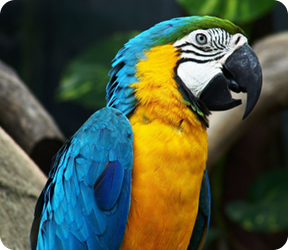
\includegraphics[scale=0.6]{figures/arara.png}
\caption{A lovely photo of an arara.}
\label{fig:arara}
\end{figure}

Lovely bird, isn't it? Now, you are probably wondering why I chose this name. Well, araras are colorful, noisy,
naughty and very funny. Everybody loves araras. So why can't you love a tool with the very same name? And
there is also another motivation of the name \emph{arara}: the chatroom residents of 
\href{http://chat.stackexchange.com/rooms/41}{\TeX.sx} -- including myself -- are fans of palindromes,
especially palindromic numbers. As you can already tell, \emph{arara} is a palindrome.

\section{How does it work?}
\label{sec:howdoesitwork}

Now that we know what \arara is, let's take a look on how the tool actually works. The whole idea is pretty
straightforward, but some concepts might be confusing at first. Do not despair, we will come back to
them later on in the manual, in Chapter~\ref{chap:importantconcepts}.

First of all, we need to add at least one instruction in the source code to tell \arara what to do. This instruction
is named \emph{directive} and it will be parsed during the preparation phase. By default, an \arara directive is
defined in a line of its own, started with a comment, followed by the word |arara:|  and the name of the task.
Code~\ref{code:hellolatex} has one directive, referencing |pdflatex|. It's important to observe that |pdflatex|
is not the command to be executed, but the name of the rule associated with that directive.

Once \arara finds a directive, it will look for the associated \emph{rule}. In our example, it will look for a rule named
|pdflatex| which will evidently run the |pdflatex|  command line application. The rule is analyzed, all possible
parameters are defined, the command line call is built and then it goes to a queue of commands to be executed.

After extracting all directives from a source code and mapping each one of them to their respective rules, \arara
then executes the queue of commands. The execution chain requires that the command $i$ was successfully
executed to then proceed to the command $i+1$, and so forth. This is also by design: \arara will halt the execution
if any of the commands in the queue had raised an error. If we run \arara on |mydoc.tex| -- we can also run
|arara mydoc| too, we will discuss this later on -- presented in Code~\ref{code:hellolatex}, we get the output
presented in Code~\ref{code:araraoutputexample}.

\begin{code}[htbp]
\caption{Running \arara on \mycmd{mydoc.tex}.}
\label{code:araraoutputexample}
\begin{bash}
$ arara mydoc
  __ _ _ __ __ _ _ __ __ _
 / _` | '__/ _` | '__/ _` |
| (_| | | | (_| | | | (_| |
 \__,_|_|  \__,_|_|  \__,_|

Running PDFLaTeX... SUCCESS
\end{bash}
\end{code}

That is pretty much how \arara works: directives in the source code are mapped to rules, which are converted to
commands and added to a queue. The queue is then executed and the status is reported. We will cover more details
about the expansion process later on in the manual. In short, we teach \arara to do a task by providing a rule,
and tell it to execute it via directives in the source code.

\section{Features}
\label{sec:features}

To name a few features I like in \arara, I'd mention the ability to write rules in a human-readable format called YAML,
which rhymes with the word \emph{camel}. YAML is actually a recursive acronym for \emph{YAML Ain't Markup Language},
and it's known as a human friendly data serialization standard for all programming languages~\cite{yaml:2001}. So far,
I think this format is quite suitable to write rules, specially if you want to avoid the need of writing complicated XML mappings or
even injecting code directly into the application.

Another feature worth mentioning is the fact that \arara is platform independent. The application was written in Java,
so \arara runs on top of a Java virtual machine, available on all the major operating systems~--~in some cases, you
might need to install the proper virtual machine. We tried very hard to keep both code and libraries compatible with
older virtual machines or from other vendors. Currently, \arara is known to run on Oracle's Java 5, 6 and 7, and OpenJDK 6 and 7.
In Chapter~\ref{chap:buildingfromsources}, there are instructions on how to build \arara from sources. Even if
you use multiple operating systems, \arara should behave the same, including the rules. There are helper functions
available in order to provide support for system-specific rules based on the underlying operating system, presented
in Section~\ref{sec:functions}.

From version 3.0 on, \arara can now display localized messages. The default language is set to English, but the user can
receive feedback from the execution process and logging in other languages as well, such as Brazilian Portuguese, German,
Italian, French, Spanish and Turkish. There's also a way to redefine the default language by adding an entry in the configuration
file, discussed later on in Section~\ref{sec:language}.

Speaking of which, \arara has now an optional configuration file in which we can add rule paths, set the default language and
define custom extensions and directive patterns, located in the user home directory. That way, we can extend \arara's behaviour
to deal with other extensions, such as |.c| files, and use the tool with other formats. We will come back on this subject later on
in Chapter~\ref{chap:configurationfile}.

\arara is also easily integrated with other \TeX\ integrated development environment, such as \TeX works~\cite{texworks:2009}, an 
environment for authoring \TeX\ documents shipped with both \TeX\ Live and MiK\TeX. Chapter~\ref{chap:ideintegration} covers
the integration of \arara with several environments.

\section{Common uses}
\label{sec:commonuses}

\arara can be used in complex workflows, like theses and books. You can tell \arara to compile the document, generate
indices and apply styles, remove temporary files, compile other |.tex| documents, create glossaries, call |pdfcrop|, move files,
run \hologo{METAPOST} or \hologo{METAFONT}, and so forth. You can easily come up with your own rules.

There's an \href{http://latex-community.org/know-how/435-gnuplot-arara}{article} available in the \LaTeX\ community which
describes the integration of |gnuplot| and \arara~\cite{cereda:2012}. This article was submitted as an entry to a contest organized
by Stefan Kottwitz. It might be worth a read.

Let's see a few examples. Code~\ref{code:exlatexone} contains the workflow I used for another article I recently wrote. Note that the first call to
|pdflatex| creates the |.aux| file, then |bibtex| will extract the cited publications. The next calls to |pdflatex| will insert
and refine the references.

\begin{code}[htbp]
\caption{\mycmd{article.tex}}
\label{code:exlatexone}
\begin{latex}
% (*@@*)arara: pdflatex
% (*@@*)arara: bibtex
% (*@@*)arara: pdflatex
% (*@@*)arara: pdflatex
\documentclass[journal]{IEEEtran}
...
\end{latex}
\end{code}

Code~\ref{code:exlatextwo} contains another workflow I used for a manual. I had to use a package that required shell escape,
so the calls to |pdflatex| had to enable it. Also, I had an index with a custom formatting, then |makeindex| was called with the
 proper style.

\begin{code}[htbp]
\caption{\mycmd{manual.tex}}
\label{code:exlatextwo}
\begin{latex}
% (*@@*)arara: pdflatex: { shell: yes }
% (*@@*)arara: makeindex: { style: mystyle }
% (*@@*)arara: pdflatex: { shell: yes }
% (*@@*)arara: pdflatex: { shell: yes }
\documentclass{book}
...
\end{latex}
\end{code}

And of course, the \arara user manual is also compiled with |arara|. You can take a look in the source code and check the
header. By the way, note that I had to use a trick to avoid |arara| to read the example directives in this manual. As we will
see later, \arara reads directives everywhere. Actually, I could have changed the directive pattern for |.tex| files through
the configuration file, but that's another story.

Other workflows can be easily created. There can be an arbitrary number of instructions for \arara to execute, so feel free to
come up with your own workflow. \arara will handle it for you. My friend Joseph Wright wrote a great article about \arara in
his personal blog, it's really worth a read~\cite{wright:2012}.

I really hope you like my humble contribution to the \TeX\ community. Let \arara enhance your \TeX\ experience, it will help you
when you'll need it the most. Enjoy the manual.

\printbibliography[heading=subbibliography]

\chapter{Installation}
\label{chap:installation}

\epigraph{\emph{Adjust \texttt{\string\hsize}: old man Fermat couldn't.}}{Enrico Gregorio}

Spledid, so you decided to give \arara a try? This chapter will cover the installation procedure. We basically
have two methods of installing \arara: the first one is through a cross-platform installer, which is of course
the recommended method; the second one is a manual deployment, with the provided |.jar| file -- a
self-contained, batteries-included executable Java archive file. If you have a recent \TeX\ Live distribution,
good news: \arara is already available in your system!

\section{Prerequisites}
\label{sec:prerequisites}

I know I've mentioned this before in Section~\ref{sec:features} and, at the risk of being repetitive, there we
go again: \arara is written in Java and thus depends on a virtual machine in the underlying operating system.
If you use a Mac or even a fairly recent Linux distribution, I have good news for you: it's mostly certain that
you already have a Java virtual machine installed.

It's very easy to check if you have a Java virtual machine installed: try running |java -version| in the terminal
(bash, command prompt, you name it) and see if you get an output similar to the one provided in
Code~\ref{code:javainstalled}.

\begin{code}[htbp]
\caption{Checking if \mycmd{java} is installed.}
\label{code:javainstalled}
\begin{bash}
$ java -version
java version "1.6.0_24"
OpenJDK Runtime Environment (IcedTea6 1.11.1)
OpenJDK Client VM (build 20.0-b12, mixed mode)
\end{bash}
\end{code}

If the output goes along the lines of |java: command not found|, I'm afraid you don't have a Java virtual
machine installed in your operating system. Since the virtual machine is a prerequisite for \arara to run,
you can install one via your favorite package manager or manually install it from the binaries available
in the official \href{http://www.java.com}{Java website}. Make sure to download the correct version for
your operating system. The installation procedure is very straightforward. If you get stuck, take a look
on the installation instructions.

It's important to mention that \arara runs also with the Java virtual machine from the OpenJDK
project~\cite{openjdk:2006}, which is already available in most of the recent Linux distributions -- actually
the output from Code~\ref{code:javainstalled} shows the OpenJDK version from my Fedora machine.
Feel free to use the virtual machine you feel most comfortable with.

Speaking of virtual machines, \arara requires at least Java 5 to run. Don't worry, it's quite easy to spot the Java
version: just look at the second digit of the version string. For example, Code~\ref{code:javainstalled} outputs |1.6.0_24|, 
which means we have Java 6 installed.

\section{Obtaining \texorpdfstring{\arara}{arara}}
\label{sec:obtainingarara}

Before proceeding, we need to choose the installation method. We have two options: the first option is the easiest one,
which installs \arara through a cross-platform installer; the second option is a manual deployment.

From version 3.0 on, \arara is also available as part of the \TeX\ Live distribution. If you have a recent \TeX\ distro,
it's almost certain that you already have \arara; make sure to select it in the |tlmgr| application.

If we opt for the installer, go to the \href{http://github.com/cereda/arara/downloads}{downloads} section of the project
 repository and download |arara-3.0-installer.jar| for all operating systems or |arara-3.0-installer.exe| for Windows.
Please note that the |.exe| version is only a wrapper which will launch |arara-3.0-installer.jar| under the hood. The 
installer also requires Java.

If we want to do things the complicated way, go to the \href{http://github.com/cereda/arara/downloads}{downloads}
section of the project repository and download the |arara.jar| file, which is a self-contained, batteries-included executable
Java archive file.

In case you want to build \arara from source, please refer to Chapter~\ref{chap:buildingfromsources} which will
cover the whole process. Thanks to Apache Maven, the build process is very easy.

\section{Using the cross-platform installer}
\label{sec:usingthecrossplatforminstaller}

After downloading |arara-3.0-installer.jar| (or its |.exe| counterpart), it's now just a matter of running it.
The installer is built with IzPack~\cite{izpack:2001}, an amazing tool for packaging applications on the Java 
platform. Of course the source is also available at the project repository. Personally, I suggest you to run the
installer in privileged mode, but you can also run it in user mode -- just keep in mind that some features might
not work, like creating symbolic links or adding the application to the system path, which inevitably requires a
privileged mode.

When running |arara-3.0-installer.jar| or its |.exe| wrapper on Windows by simply double-clicking it, the installer
will automatically run in privileged mode. A general Unix-based installation can be triggered by the command
presented in Code~\ref{code:runinstaller1}. There's also an alternative command presented in 
Code~\ref{code:runinstaller2}.

\begin{code}[htbp]
\caption{Running the installer in a Unix-based system -- method 1.}
\label{code:runinstaller1}
\begin{bash}
$ sudo java -jar arara-3.0-installer.jar
\end{bash}
\end{code}

\begin{code}[htbp]
\caption{Running the installer in a Unix-based system -- method 2.}
\label{code:runinstaller2}
\begin{bash}
$ su -c 'java -jar arara-3.0-installer.jar'
\end{bash}
\end{code}

Since Windows doesn't have a similar command to |su| or |sudo|, you need to open the command prompt as
administrator and then run the command presented in Code~\ref{code:runinstallerwin}. You can right-click
the command prompt shortcut and select the ``Run as administrator\ldots'' option.

\begin{code}[htbp]
\caption{Running the installer in the Windows command prompt as administrator.}
\label{code:runinstallerwin}
\begin{bash}
C:\> java -jar arara-3.0-installer.jar
\end{bash}
\end{code}

The installation process will begin. Hopefully, the first screen of the installer will appear, which is the
language selection (Figure~\ref{fig:instlang}). By the way, if you called the installer through the command line,
please do not close the terminal! It might end the all running processes, including our installer.

\begin{figure}[htbp]
\centering
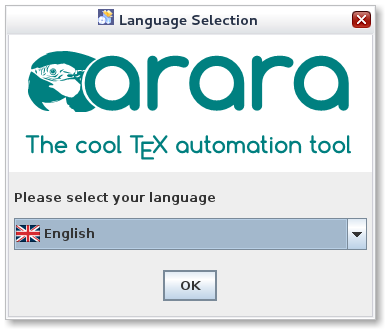
\includegraphics[scale=0.5]{figures/install-langsel.png}
\caption{Language selection screen.}
\label{fig:instlang}
\end{figure}

% TODO add more languages
The installer currently supports six languages: English, German, French, Italian, Spanish, and Brazilian Portuguese.
I plan to add more languages to the list in the near feature.

The next screen welcomes you to the installation (Figure~\ref{fig:instwelcome}). There's the application name, the
current version, the team, and the project homepage. We can proceed by clicking the \textit{Next} button. 
Note that you can quit the installer at any time by clicking the \textit{Quit} button -- please, don't do it; a kitten dies
every time you abort the installation\footnote{Of course, this statement is just a joke. No animals were 
harmed, killed or severely wounded during the making of this user manual. After all, \arara is environmentally friendly.}.

\begin{figure}[htbp]
\centering
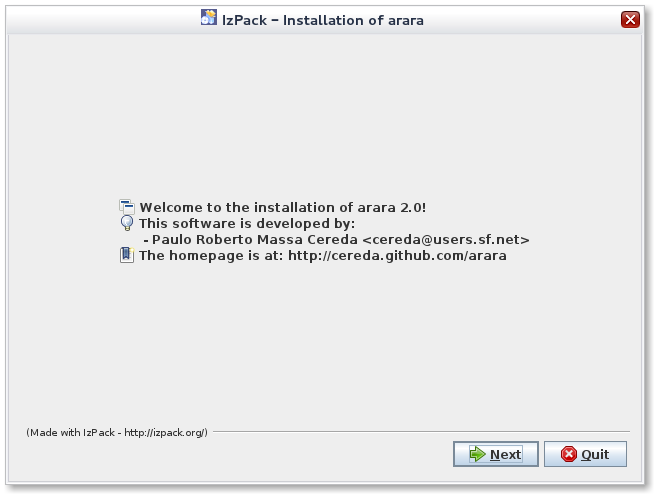
\includegraphics[scale=0.5]{figures/install-welcome.png}
\caption{Welcome screen.}
\label{fig:instwelcome}
\end{figure}

Moving on, the next screen shows the license agreement (Figure~\ref{fig:instlicense}). \arara is licensed under the 
\href{http://www.opensource.org/licenses/bsd-license.php}{New BSD License}~\cite{bsd:2012}. It's important to
observe that the New BSD License has been verified as a GPL-compatible free software license by the Free Software
Foundation~\cite{fsf:1985}, and has been vetted as an open source license by the Open Source Initiative~\cite{osi:1998}.
The full license is also available in this document (page~\pageref{sec:license}). You need to accept the terms of the 
license agreement before proceeding.

The next screen is probably the most important section of the installation: in here we will choose the packs we want to
install (Figure~\ref{fig:instpacks}). All packs are described in Table~\ref{tab:packs}. Note that the grayed packs are 
required.

\begin{figure}[htbp]
\centering
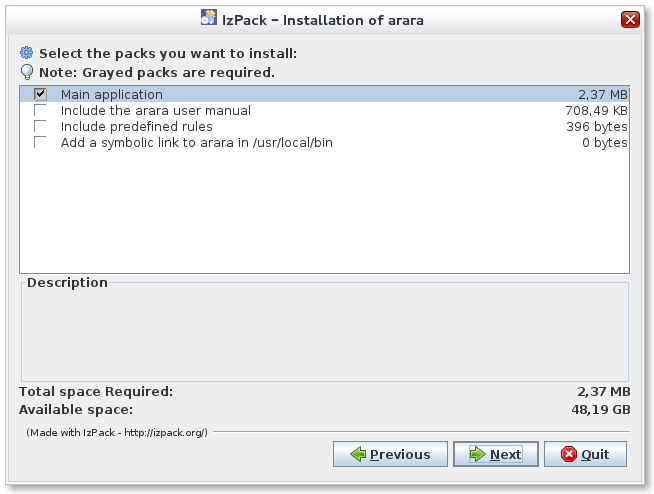
\includegraphics[scale=0.5]{figures/install-packs.png}
\caption{Packs screen.}
\label{fig:instpacks}
\end{figure}

\begin{table}[htbp]
\centering
\caption{Available packs.}
\label{tab:packs}
\renewcommand{\arraystretch}{1.5}
\footnotesize
\begin{tabular}{p{0.30\textwidth}p{0.12\textwidth}p{0.4\textwidth}}
\hline
\textbf{Pack name} & \textbf{OS} & \textbf{Description}                       \\
\hline
\hline
Main application & All & This pack contains the core application. It also 
provides an |.exe| wrapper for Windows and a bash file for Unix.              \\
\hline
Include the \arara user manual & All & This pack installs this user manual into 
the |docs/| subdirectory of \arara.                                           \\
\hline
Include predefined rules & All & Of course, \arara has a set of predefined rules
for you to start with. If you prefer to write your own rules from scratch, do 
not select this pack.                                                         \\
\hline
Add a symbolic link to \arara in |/usr/local/bin| & Unix & If you ran the 
installer in privileged mode, a symbolic link to \arara can be created in the 
|/usr/local/bin| directory. There's no magic here, the installer uses the good 
old |ln| command.                                                             \\
\hline
Add \arara to the system path & Windows & Like the Unix task, \arara can also 
add itself to the system path. This feature is provided by a Windows script named
\href{http://legroom.net/software/modpath}{Modify Path}~\cite{modpath:2012}. \\
\hline
\end{tabular}
\end{table}

It's very important to mention that all these modifications in the operating 
system -- the symbolic link creation for Unix or the addition to the path for 
Windows -- are safely removed when you run the \arara uninstaller. We will talk 
about it later, in Section~\ref{sec:uninstallingarara}.

\begin{figure}[htbp]
\centering
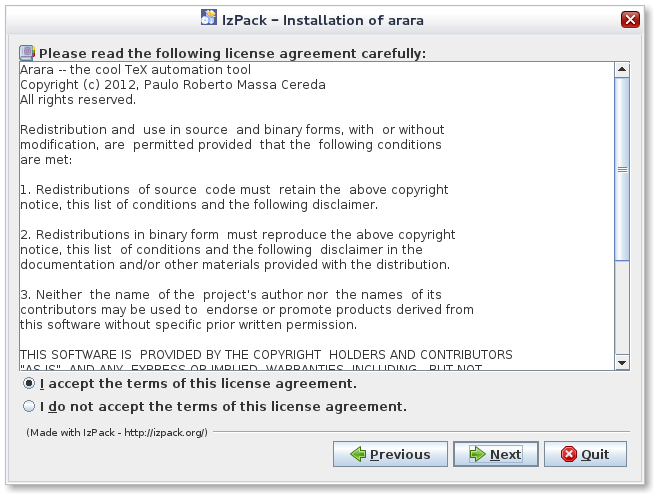
\includegraphics[scale=0.5]{figures/install-license.png}
\caption{License agreement screen.}
\label{fig:instlicense}
\end{figure}

In the next screen, we will select the installation path (Figure~\ref{fig:instpath}). The installer
will automatically set the default installation path according to the Table~\ref{tab:paths}, but
feel free to install \arara in your favorite structure -- even |/opt| or your home folder.

\begin{table}[htbp]
\centering
\caption{Default installation paths.}
\label{tab:paths}
\renewcommand{\arraystretch}{1.5}
\begin{tabular}{cl}
\hline
\textbf{OS} & \textbf{Default installation path}\\
\hline
\hline
Windows & |C:\Program Files\arara|\\
Unix & |/usr/local/arara|\\
\hline
\end{tabular}
\end{table}

\begin{figure}[htbp]
\centering
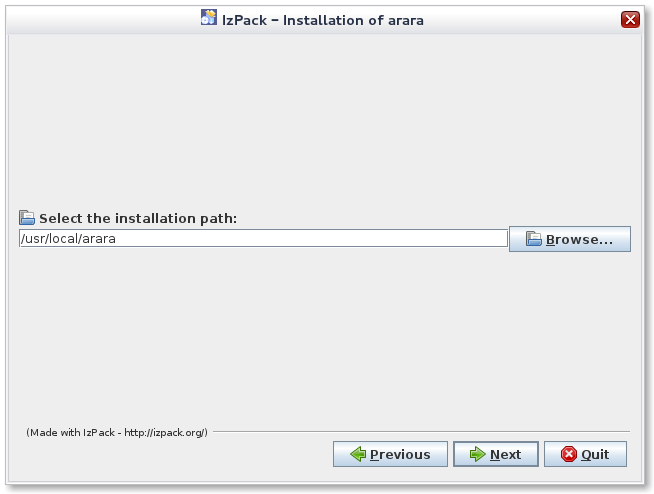
\includegraphics[scale=0.5]{figures/install-path.png}
\caption{Installation path screen.}
\label{fig:instpath}
\end{figure}

After selecting the installation path, the installer will then confirm the creation of the target directory
(Figure~\ref{fig:instnewfolder}). We simply click \textit{OK} to accept it. For convenience, the full installation path 
defined in the installation path screen (Figure~\ref{fig:instpath}) will be referred as |ARARA_HOME| from now on.

\begin{figure}[htbp]
\centering
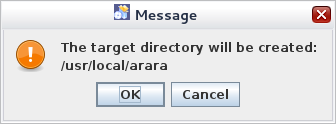
\includegraphics[scale=0.5]{figures/install-pathwarning.png}
\caption{Target directory confirmation.}
\label{fig:instnewfolder}
\end{figure}

Now, just sit back and relax while \arara is being installed (Figure~\ref{fig:instprogress}). All selected packs will
be installed accordingly. The post installation tasks -- like creating the symbolic link or adding \arara to the system
path -- are performed here as well. If the installation has completed successfully, we will reach the final screen of
the installer congratulating us for installing \arara (Figure~\ref{fig:instfinish}).

\begin{figure}[htbp]
\centering
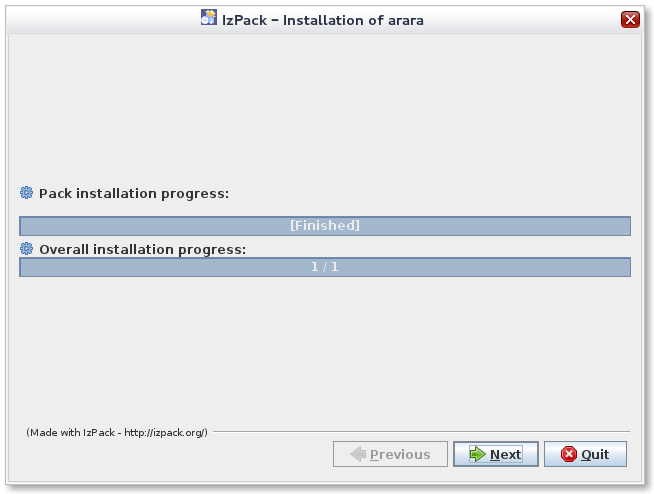
\includegraphics[scale=0.5]{figures/install-progress.png}
\caption{Progress screen.}
\label{fig:instprogress}
\end{figure}

\begin{figure}[htbp]
\centering
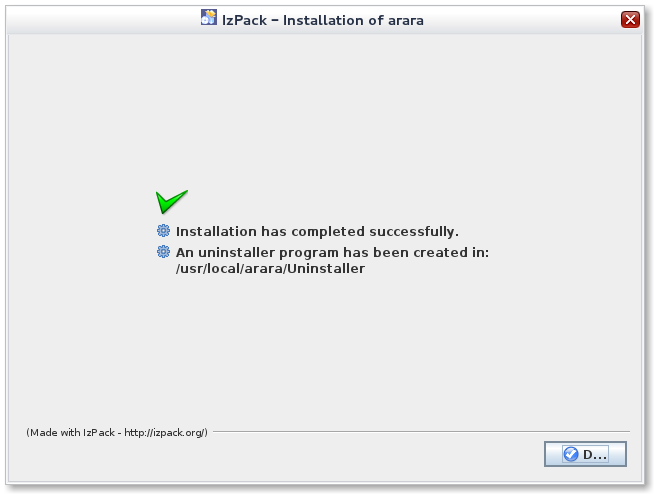
\includegraphics[scale=0.5]{figures/install-finish.png}
\caption{Final screen.}
\label{fig:instfinish}
\end{figure}

The full installation scheme is presented in Figure~\ref{fig:ararastructure}. The directory structure is
presented here as a whole; keep in mind that some parts will be omitted according to your operating
system and pack selection. For example, the |etc/| subdirectory will only be installed if and only if
you are in Windows and the system path pack is selected. Other files are platform-specific, such as
|arara.exe| for Windows and the |arara| bash file for Unix.

\begin{figure}[htbp]
\centering
\begin{tikzpicture}[grow via three points={one child at (0.5,-0.7) and two children at (0.5,-0.7) and (0.5,-1.4)}, edge from parent path={(\tikzparentnode.south) |- (\tikzchildnode.west)}, anchor=west, font=\ttfamily]
  \node {ARARA\_HOME/}
    child { node {arara.jar}}		
    child { node {arara.exe}}
    child { node {arara}}
    child { node {docs/}
      child { node {arara-usermanual.pdf}}
    }
    child [missing] {}
    child { node {etc/}
      child { node {modpath.exe}}
    }
    child [missing] {}
    child { node {Uninstaller/}
      child { node {uninstaller.jar}}
    }
	child [missing] {}
	  child { node {rules/}
        child { node {biber.yaml}}
        child { node {\ldots}}
        child { node {xetex.yaml}}
    };
\end{tikzpicture}
\caption{Installation scheme.}
\label{fig:ararastructure}
\end{figure}

That's it, \arara is installed in your operating system. If you opted for the symbolic link creation or the path addition,
\arara is already available in your terminal by simply typing |arara|. Have fun!

\section{Manual installation}
\label{sec:manualinstallation}

Thankfully, \arara is also very easy to be manually deployed. First of all, we must create the application directory.
Feel free to create this directory anywhere in your computer; it can be |C:\arara|, |/opt/arara| or another location 
of your choice. This procedure is similar to the installation path screen (Figure~\ref{fig:instpath}) from
Section~\ref{sec:installer}. Again, for convenience, the full installation path will be referred as |ARARA_HOME| from 
now on. Although it's not mandatory, try to avoid folders structures with spaces in the path. In any case,
\arara can handle such spaces.

After downloading |arara.jar| from the \href{http://github.com/cereda/arara/downloads}{downloads} section of
the project repository, let's copy it to the |ARARA_HOME| directory we've created in the previous step.
Since |arara.jar| is a self-contained, batteries-included executable Java archive file, \arara is already installed.

In order to run \arara from a manual installation, we should open a terminal and run |java -jar $ARARA_HOME/arara.jar|,
but that is far from being intuitive. To make our lives easier, we will create a shortcut for this
command.

If you are deploying \arara in Windows, there are two methods for creating a shortcut: the first method -- the
easiest -- consists of downloading the |arara.exe| wrapper from the \href{http://github.com/cereda/arara/downloads}{downloads}
section and copying it to the |ARARA_HOME| directory, in the same level of |arara.jar|. This |.exe| wrapper, provided by \href{http://launch4j.sourceforge.net}{Launch4J}~\cite{launch4j:2005}, wraps |.jar| files in Windows native executables
and allows to run them like a regular Windows program.

The second method for creating a shortcut in Windows is to provide a batch file which will call |java -jar $ARARA_HOME/arara.jar|
for us. Create a file named |arara.bat| or |arara.cmd| inside the |ARARA_HOME| directory, in the same level of |arara.jar|, and
add the content from Code~\ref{code:windows}.

\begin{code}[htbp]
\caption{Creating a batch file for \arara in Windows.}
\label{code:windows}
\begin{bash}
@echo off
java -jar "%~dp0\arara.jar" %*
\end{bash}
\end{code}

After creating the batch file, add the full |ARARA_HOME| path to the system path. Unfortunately, this manual can't cover
the path settings, since it's again a matter of personal taste. I'm sure you can find tutorials on how to add a directory to
the system path.

If you are deploying \arara in Linux or Mac, we also need to create a shortcut to |java -jar $ARARA_HOME/arara.jar|.
Create a file named |arara| inside the |ARARA_HOME| directory, in the same level of |arara.jar|, and add the content 
from Code~\ref{code:unix}.

\begin{code}[htbp]
\caption{Creating a script for \arara in Linux and Mac.}
\label{code:unix}
\begin{bash}
#!/bin/bash
# Example script of arara
# Installation and usage are described in the documentation
SOURCE="${BASH_SOURCE[0]}"
while [ -h "$SOURCE" ] ; do SOURCE="$(readlink "$SOURCE")"; done
DIR="$( cd "$( dirname "${BASH_SOURCE[0]}" )" && cd -P "$( dirname "$SOURCE" )" && pwd )"
java -jar "$DIR/arara.jar" "$@"
\end{bash}
\end{code}

We now need to add execute permissions for our newly created script through |chmod +x arara|. The |arara| script can
be invoked through path addition or symbolic link. I personally prefer to add |ARARA_HOME| to my user path, but a
symbolic link creation seems way more robust -- it's what the installer does. Anyway, it's up to you to decide which method
you want to use. There's no need to use both.

Once we conclude the manual installation, it's time to check if \arara is working properly. Try running |arara| in the terminal
and see if you get the output shown in Code~\ref{code:arararun}.

\begin{code}[p]
\caption{Testing if \arara is working properly.}
\label{code:arararun}
\begin{nolanguage}
$ arara 
  __ _ _ __ __ _ _ __ __ _ 
 / _` | '__/ _` | '__/ _` |
| (_| | | | (_| | | | (_| |
 \__,_|_|  \__,_|_|  \__,_|

arara 3.0 - The cool TeX automation tool
Copyright (c) 2012, Paulo Roberto Massa Cereda
All rights reserved.

usage: arara [file [--log] [--verbose] [--timeout N] [--language L] | --help | --version]

 -h,--help             print the help message
 -L,--language <arg>   set the application language
 -l,--log              generate a log output
 -t,--timeout <arg>    set the execution timeout (in milliseconds)
 -v,--verbose          print the command output
 -V,--version          print the application version
\end{nolanguage}
\end{code}

If the terminal doesn't display the \arara logo and usage, please review the manual installation steps.
Every step is important in order to make \arara available in your system. You can also try the cross-platform
installer. If you still have any doubts, feel free to contact us.

\section{Updating \texorpdfstring{\arara}{arara}}
\label{sec:updatingarara}

If there is a newer version of \arara available in the \href{http://github.com/cereda/arara/downloads}{downloads}
section of the project repository, simply download the |arara.jar| file and copy it to the |ARARA_HOME| directory,
replacing the current one. No further steps are needed, the newer version is deployed. Try running |arara --version|
in the terminaland see if the version shown in the output is equal to the one you have downloaded.

Anyway, for every version, \arara has the proper cross-platform installer available for download in the project repository.
You can always uninstall the old \arara setup and install the new one. Please note that only major versions are released
with the installer.

If you have \arara through the \TeX\ Live distribution, the update process is straightforward: simply open a
terminal and run |tlmgr update arara| in order to update the application. This is of course the preferred method.

\section{Uninstalling \texorpdfstring{\arara}{arara}}
\label{sec:uninstallingarara}

If you want to uninstall \arara, there are two methods available. If you installed \arara through the cross-platform installer,
I have good news for you: it's just a matter of running the uninstaller. Now, if \arara was deployed through the manual
installation, we might have to remove some links or path additions.

A general Unix-based uninstallation can be triggered by the command presented in Code~\ref{code:uninstall1}.
There's also an alternative command presented in Code~\ref{code:uninstall2}.

\begin{code}[htbp]
\caption{Running the uninstaller in a Unix-based system -- method 1.}
\label{code:uninstall1}
\begin{bash}
$ sudo java -jar $ARARA_HOME/Uninstaller/uninstaller.jar
\end{bash}
\end{code}

\begin{code}[htbp]
\caption{Running the uninstaller in a Unix-based system -- method 2.}
\label{code:uninstall2}
\begin{bash}
$ su -c 'java -jar $ARARA_HOME/Uninstaller/uninstaller.jar'
\end{bash}
\end{code}

Since Windows doesn't have a similar command to |su| or |sudo|, you need to open the command prompt as administrator
and then run the command presented in Code~\ref{code:uninstallwin}. You can right-click the command prompt shortcut 
and select the ``Run as administrator\ldots'' option.

\begin{code}[htbp]
\caption{Running the uninstaller in the Windows command prompt as administrator.}
\label{code:uninstallwin}
\begin{bash}
C:\> java -jar $ARARA_HOME/Uninstaller/uninstaller.jar
\end{bash}
\end{code}

The uninstallation process will begin. Hopefully, the first and only creen of the uninstaller will appear
(Figure~\ref{fig:uninstallone}). By the way, if you called the uninstaller through the command line, please
do not close the terminal! It might end the all running processes, including our uninstaller.

\begin{figure}[htbp]
\centering
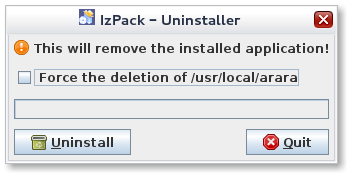
\includegraphics[scale=0.5]{figures/uninstall-welcome.png}
\caption{The uninstaller screen.}
\label{fig:uninstallone}
\end{figure}

There's nothing much to see in the uninstaller. We have an option to force the deletion of the |ARARA_HOME| directory,
but that's all. By clicking the \textit{Uninstall} button, the uninstaller will remove the symbolic link or the path entry for
\arara from the operating system, if selected during the installation. Then it will erase the |ARARA_HOME| directory 
(Figure~\ref{fig:uninstalltwo}).

\begin{figure}[htbp]
\centering
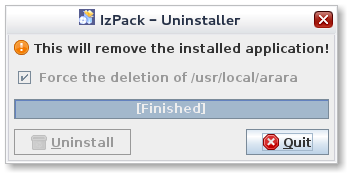
\includegraphics[scale=0.5]{figures/uninstall-finish.png}
\caption{The uninstaller screen, after the execution.}
\label{fig:uninstalltwo}
\end{figure}

Unfortunately, even if you force the deletion of the |ARARA_HOME| directory in Windows, the operating system can't
remove the |Uninstaller| subdirectory because the uninstaller was being executed from there. But that's the only trace 
left. You can safely delete |ARARA_HOME| after running the uninstaller.

If \arara was manually installed, we need to remove the symbolic link reference or the path entry, if any, then delete
the |ARARA_HOME| directory. Don't leave any traces of \arara in system directories or configuration files; a broken 
symbolic link or a wrong path entry might cause trouble in the future.

\printbibliography[heading=subbibliography]

\chapter{Building from sources}
\label{chap:buildingfromsources}

\section{Obtaining the sources}
\label{sec:obtainingthesources}

\section{Building \texorpdfstring{\arara}{arara}}
\label{sec:buildingarara}

\section{Notes on the installer and wrapper}
\label{sec:notesontheinstallerandwrapper}

\chapter{IDE integration}
\label{chap:ideintegration}

\section{TeXworks}
\section{TeXnic Center}
\section{Kile}
\section{TeXmaker}
\section{TeXstudio}
\section{WinEdt}
\section{Inlage}
\section{TeXShop}

\chapter{Important concepts}
\label{chap:importantconcepts}

\section{Rules}
\label{sec:rules}

\section{Directives}
\label{sec:directives}

\section{Orb tags}
\label{sec:orbtags}

\chapter{Configuration file}
\label{chap:configurationfile}

\section{Search paths}
\label{sec:searchpaths}

\section{Language}
\label{sec:language}

\section{File patterns}
\label{sec:filepatterns}

\chapter{Running arara}
\section{Command line}
\section{Messages}
\section{Command output}
\section{Logging}

\part{For authors}

\chapter{Quick start}
\section{Predefined rules}
\section{Organizing directives}
\section{Best practices}

\chapter{Reference for rule library}
\label{chap:referenceforrulelibraryone}

\section{Directives and arguments}
\label{sec:directivearguments}

\section{Special orb tags}
\label{sec:specialorbtags}

\part{For rulemakers}

\chapter{Quick start}
\section{Writing rules}
\section{Cross-platform rules}
\section{Best practices}

\chapter{Reference for rule library}
\label{chap:referenceforrulelibrarytwo}

\section{Functions}
\label{sec:functions}

\section{Notes on expansion}
\label{sec:notesonexpansion}

\part{Structure and execution}

\chapter{Inside the rule format}
\section{Available fields}
\section{Expansion order}
\section{Processing rules}

\chapter{Inside the application}
\section{Looking for directives}
\section{Mapping directives to rules}
\section{Executing commands}

\end{document}
